\subsection{NUMA}
Pour dépasser les limites de l'architecture SMP, la mémoire peut être physiquement distribuée entre chaque processeur (Fig.~\ref{fig:numa}).
%
Avec l'architecture NUMA, la latence et la bande passante de chaque accès mémoire dépendent de la distance entre le processeur qui fait la demande et la position physique de la mémoire.
%
Il existe différents moyens d'inter-connecter les processeurs, on peut connecter tous les processeurs un à un pour faire en sorte que la latence soit la plus faible possible, mais tout comme l'architecture SMP cette méthode ne passe pas à l'échelle.
%
Il est aussi possible de limiter le nombre de connexions par processeur tout en optimisant le nombre maximum de sauts, comme fait dans les grappes de calcul.

La distance entre chaque banc NUMA est fournie par le constructeur de la machine sous la forme d'une matrice de distance.
%
Nous pouvons utiliser cette matrice pour retrouver la topologie des noeuds NUMA de la machine.
%
La puissance théorique est la même que pour une machine SMP, mais en pratique nous obtenons de meilleures performances.
%
En contrepartie, pour obtenir ces performances, il est nécessaire d'avoir une bonne gestion de la mémoire.
%
Cette gestion peut-être faite par le noyau du système d'exploitation puis affinée par le programme lui-même.
%
La plupart des machines NUMA sont ccNUMA\footnote{cache coherent NUMA}, c'est-à-dire que les caches de données sont cohérents entre chaque processeur.
%
Les machines que nous allons utiliser sont toutes ccNUMA, cela signifie qu'une écriture sur un banc NUMA distant coûtera plus cher qu'une lecture.

%   (-_-)   %
\begin{figure}[!h]
  \centering
  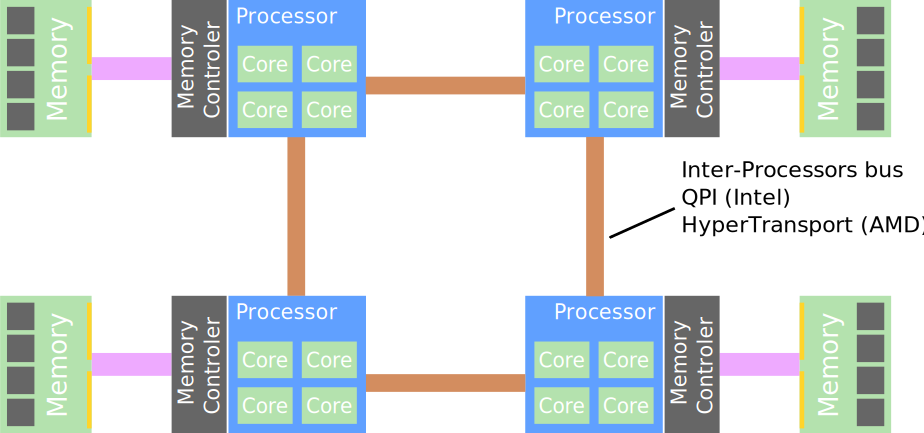
\includegraphics[width=0.8\textwidth]{numa}
  \caption{Vue d'ensemble d'une architecture NUMA.}
  \label{fig:numa}
\end{figure}
